
%------------------------------------------------   
\section{Clustering}

La aplicación de técnicas de clustering permite obtener agrupaciones y relaciones en los datos que a simple vista no se pueden obtener. En esta sección se va a realizar la aplicación del algoritmo de clustering K-Means \citep{scikit-learn}, realizando primero un preprocesamiento de los datos y posteriormente la obtención de algunas métricas sobre los clusters obtenidos. Todo esto se encuentra implementado en el notebook \\ \code{src/clustering-and-data-analysis.ipynb} \citep{master}.


%------------------------------------------------   
\subsection{Preprocesamiento}
\label{sec:clustering-preprocessing}

Antes de poder aplicar el algoritmo de clustering K-Means \citep{scikit-learn}, el dataset debe ser preprocesado. El preprocesamiento de este dataset ha consistido en los siguientes pasos:

\begin{itemize}
 \item \textbf{Rellenar valores nulos}. En el dataset se han encontrado tres tipos de valores nulos: 
 \begin{itemize}
  \item \textbf{Valores de formato fecha}. Han sido rellenados con el valor \code{01/01/1990}.
  \item \textbf{Valores de formato texto}. Han sido rellenados con el valor de la cadena vacía.
  \item \textbf{Valores de formato texto asociados a identificadores}. Han sido rellenados con el valor \code{-1}.
 \end{itemize}
 
 \item \textbf{Eliminar de los registros} con valor distinto de \code{01/01/1990} en los campos \\ \code{DiscontinuedDate} y \code{ChemicalDateRemoved}, pues solo se precisan de aquellos registros de cosméticos que tengan productos químicos y no hayan sido retirados del mercado.

 \item \textbf{Seleccionar las características} expuestas en la Tabla \ref{tab:features-selection}.
 \item \textbf{Agrupar por año y mes} de cada una de las características de formato fecha, sumando los valores del campo \code{ChemicalCount}.
 \item \textbf{Seleccionar características que presenten multicolinealidad} en el dataset aplicando el Factor de Inflación de la Varianza \textit{(Variance Inflation Factor (VIF))} \citep{vif}.
\end{itemize}

Tras aplicar este preprocesamiento, el dataset resultante se compone de 7.487 registros y 7 características, las cuales se muestran en la Tabla \ref{tab:features-preprocessing}, donde \code{\_Year} y \code{\_Month} indican el año y el mes del campo asociado, respectivamente.

\begin{table}[!th]
\begin{tabular}{@{}l@{}}
\toprule
Nombre                                \\ \midrule
\code{InitialDateReported\_Year}      \\
\code{InitialDateReported\_Month}     \\
\code{MostRecentDateReported\_Year}   \\
\code{MostRecentDateReported\_Month}  \\ 
\code{SubCategoryId}                  \\
\code{CasId}                          \\ 
\code{ChemicalCount}                  \\
\bottomrule
\end{tabular}
\centering
\caption{Características del dataset después del preprocesamiento.}
\label{tab:features-preprocessing}
\end{table}





%------------------------------------------------   
\subsection{Aplicación del algoritmo K-Means}

Una vez aplicado el preprocesamiento, tenemos el dataset preparado para poder aplicar el algoritmo de clustering K-Means \citep{scikit-learn}. Sin embargo, este algoritmo necesita que se le proporcione el número de clusters en los que dividir el dataset. Con las características que presenta el dataset no se puede saber el número óptimo de clusters sin aplicar alguna técnica que nos proporcione este número. \\

Para la obtención del número óptimo de clusters, se han utilizado los métodos de la Silueta \textit{(Silhouette Method)} \citep{scikit-learn} y del Codo \textit{(Elbow Method)} \citep{elbow}. En la Figura \ref{fig:silhouette-elbow-methods} se muestran las dos gráficas de la aplicación de los métodos anteriores al dataset. Estas gráficas nos indican que el número óptimo de clusters en los que se divide el dataset es 3. \\

Una vez obtenido el número óptimo de clusters, se puede aplicar el algoritmo K-Means indicándole que el número de clusters es 3. Las Tablas \ref{tab:cluster0}, \ref{tab:cluster1}, \ref{tab:cluster1-1} y \ref{tab:cluster2} muestran la distribución de los productos químicos en los tres clusters tras aplicar el algoritmo. \\

La Figura \ref{fig:clusters-distribution} muestra la distribución de los cluster obtenidos según la relación entre los productos químicos \code{CasId} y los cosméticos \code{SubCategoryId}. Mientras que la Tabla \ref{tab:clusters-distribution} muestra la distribución de los clusters de manera numérica.


\begin{figure}[!th]
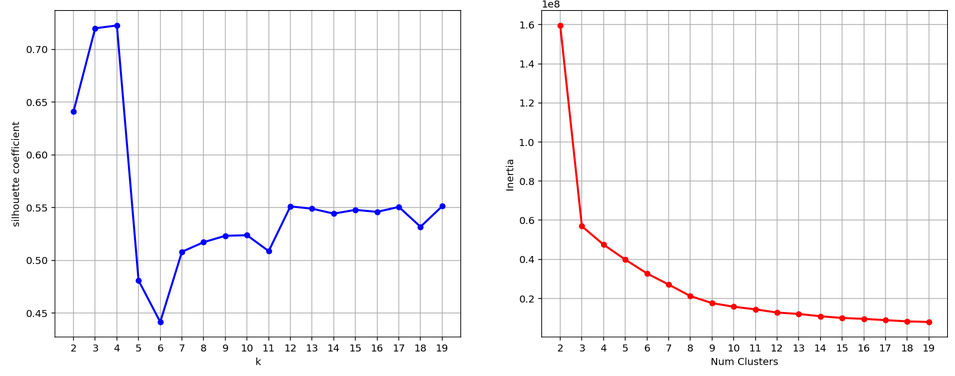
\includegraphics[scale=0.45]{figures/silhouette-elbow-methods}
\centering
\caption{Aplicación de los métodos \textit{Silhouette} (izquierda) y \textit{Elbow} (derecha) para la obtención del número óptimo de clusters.}
\label{fig:silhouette-elbow-methods}
\end{figure}

\begin{figure}[!th]
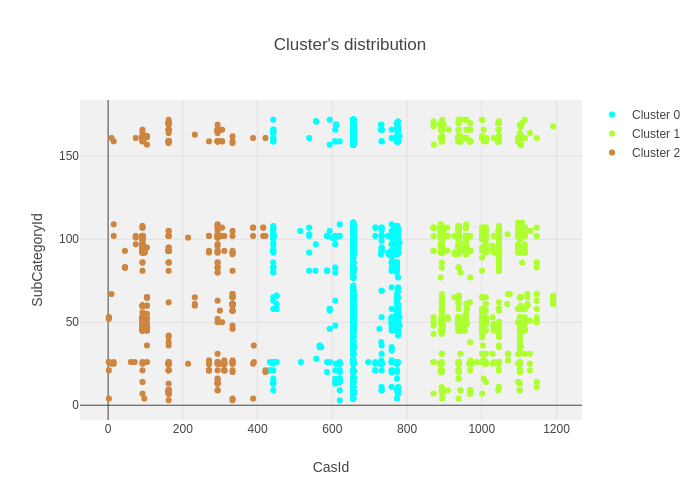
\includegraphics[scale=0.5]{figures/clusters-distribution}
\centering
\caption{Distribución de los clusters según la relación entre los productos químicos \code{CasId} y los cosméticos \code{SubCategoryId}.}
\label{fig:clusters-distribution}
\end{figure}

\begin{table}[!th]
\begin{tabular}{@{}ccc@{}}
\toprule
Cluster 0 & Cluster 1 & Cluster 2 \\ \midrule
$5532$ & $1476$ & $479$ \\
\bottomrule
\end{tabular}
\centering
\caption{Distribución de los clusters según el número de registros de cada cluster.}
\label{tab:clusters-distribution}
\end{table}



%------------------------------------------------   
\subsection{Métricas del clustering}

Tras aplicar el clustering, se van a calcular ciertas métricas sobre los clusters obtenidos para ofrecer los resultados del clustering de manera más precisa. Las métricas que han sido utilizadas son las siguientes:

\begin{itemize}
 \item \code{Average Within} \citep{metrics}. Mide la distancia media dentro de las observaciones de cada cluster (distancia intra-cluster). Viene definido por la ecuación \ref{eq:average-within}, siendo $K$ el número de clusters, $C_i$ el conjunto de elementos del cluster $i$ y $centroid_i$ el centroide del cluster $i$: 
 \begin{equation}
  SSE = \sum\limits^{K}_{i=1} \sum\limits_{x \in C_i} dist(centroid_i, x)^2
  \label{eq:average-within}
 \end{equation}
 
 \item \code{Dunn Index} \citep{metrics}. Define el ratio entre la distancia mínima inter-cluster y la máxima distancia intra-cluster. Viene definido por la ecuación \ref{eq:dunn-index}, siendo $C$ el conjunto de todos los clusters.
  \begin{equation}
  D(C) = \frac{\min\limits_{C_k, C_l \in C, C_k \neq C_l} (\min\limits_{i,j \in C_k, C_l} dist(i, j))}{\max\limits_{C_m \in C} diam(C_m)}
  \label{eq:dunn-index}
 \end{equation}
\end{itemize}

Así pues, las métricas obtenidas se muestran en la Tabla \ref{tab:metrics}:

\begin{table}[!th]
\begin{tabular}{@{}cc@{}}
\toprule
\code{Average Within} & \code{Dunn Index} \\ \midrule
$0.048633$ & $5.692750 \cdot 10^7$ \\
\bottomrule
\end{tabular}
\centering
\caption{Valores obtenidos para las métricas \code{Average Within} y \code{Dunn Index}.}
\label{tab:metrics}
\end{table}






